% *** Authors should verify (and, if needed, correct) their LaTeX system  ***
% *** with the testflow diagnostic prior to trusting their LaTeX platform ***
% *** with production work. IEEE's font choices can trigger bugs that do  ***
% *** not appear when using other class files.                            ***
% The testflow support page is at:
% http://www.michaelshell.org/tex/testflow/


%%*************************************************************************
%% Legal Notice:
%% This code is offered as-is without any warranty either expressed or
%% implied; without even the implied warranty of MERCHANTABILITY or
%% FITNESS FOR A PARTICULAR PURPOSE!
%% User assumes all risk.
%% In no event shall IEEE or any contributor to this code be liable for
%% any damages or losses, including, but not limited to, incidental,
%% consequential, or any other damages, resulting from the use or misuse
%% of any information contained here.
%%
%% All comments are the opinions of their respective authors and are not
%% necessarily endorsed by the IEEE.
%%
%% This work is distributed under the LaTeX Project Public License (LPPL)
%% ( http://www.latex-project.org/ ) version 1.3, and may be freely used,
%% distributed and modified. A copy of the LPPL, version 1.3, is included
%% in the base LaTeX documentation of all distributions of LaTeX released
%% 2003/12/01 or later.
%% Retain all contribution notices and credits.
%% ** Modified files should be clearly indicated as such, including  **
%% ** renaming them and changing author support contact information. **
%%
%% File list of work: IEEEtran.cls, New_IEEEtran_how-to.pdf, bare_jrnl_new_sample4.tex,
%%*************************************************************************
\PassOptionsToPackage{unicode}{hyperref}
\PassOptionsToPackage{hyphens}{url}
\PassOptionsToPackage{dvipsnames,svgnames,x11names}{xcolor}
% Note that the a4paper option is mainly intended so that authors in
% countries using A4 can easily print to A4 and see how their papers will
% look in print - the typesetting of the document will not typically be
% affected with changes in paper size (but the bottom and side margins will).
% Use the testflow package mentioned above to verify correct handling of
% both paper sizes by the user's LaTeX system.
%
% Also note that the "draftcls" or "draftclsnofoot", not "draft", option
% should be used if it is desired that the figures are to be displayed in
% draft mode.
%
\documentclass[
  journal,
]{IEEEtran}%
% If IEEEtran.cls has not been installed into the LaTeX system files,
% manually specify the path to it like:
% \documentclass[journal]{../sty/IEEEtran}
\usepackage[cmex10]{amsmath}
\usepackage{amssymb}
\usepackage{iftex}
\ifPDFTeX
  \usepackage[T1]{fontenc}
  \usepackage[utf8]{inputenc}
  \usepackage{textcomp} % provide euro and other symbols
\else % if luatex or xetex
  \usepackage{unicode-math} % this also loads fontspec
  \defaultfontfeatures{Scale=MatchLowercase}
  \defaultfontfeatures[\rmfamily]{Ligatures=TeX,Scale=1}
\fi
%\usepackage{lmodern}
\ifPDFTeX\else
\fi
% Use upquote if available, for straight quotes in verbatim environments
\IfFileExists{upquote.sty}{\usepackage{upquote}}{}
\IfFileExists{microtype.sty}{% use microtype if available
  \usepackage[]{microtype}
  \UseMicrotypeSet[protrusion]{basicmath} % disable protrusion for tt fonts
}{}
\makeatletter
\parindent    1.0em
\ifCLASSOPTIONcompsoc
  \parindent    1.5em
\fi
\makeatother
\usepackage{xcolor}
\setlength{\emergencystretch}{3em} % prevent overfull lines

\setcounter{secnumdepth}{5}
% Make \paragraph and \subparagraph free-standing
\ifx\paragraph\undefined\else
  \let\oldparagraph\paragraph
  \renewcommand{\paragraph}[1]{\oldparagraph{#1}\mbox{}}
\fi
\ifx\subparagraph\undefined\else
  \let\oldsubparagraph\subparagraph
  \renewcommand{\subparagraph}[1]{\oldsubparagraph{#1}\mbox{}}
\fi


\providecommand{\tightlist}{%
  \setlength{\itemsep}{0pt}\setlength{\parskip}{0pt}}\usepackage{longtable,booktabs,array}
\usepackage{calc} % for calculating minipage widths
% Correct order of tables after \paragraph or \subparagraph
\usepackage{etoolbox}
\makeatletter
\patchcmd\longtable{\par}{\if@noskipsec\mbox{}\fi\par}{}{}
\makeatother
% Allow footnotes in longtable head/foot
\IfFileExists{footnotehyper.sty}{\usepackage{footnotehyper}}{\usepackage{footnote}}
\makesavenoteenv{longtable}
\usepackage{graphicx}
\makeatletter
\def\maxwidth{\ifdim\Gin@nat@width>\linewidth\linewidth\else\Gin@nat@width\fi}
\def\maxheight{\ifdim\Gin@nat@height>\textheight\textheight\else\Gin@nat@height\fi}
\makeatother
% Scale images if necessary, so that they will not overflow the page
% margins by default, and it is still possible to overwrite the defaults
% using explicit options in \includegraphics[width, height, ...]{}
\setkeys{Gin}{width=\maxwidth,height=\maxheight,keepaspectratio}
% Set default figure placement to htbp
\makeatletter
\def\fps@figure{htbp}
\makeatother
% definitions for citeproc citations
\NewDocumentCommand\citeproctext{}{}
\NewDocumentCommand\citeproc{mm}{%
  \begingroup\def\citeproctext{#2}\cite{#1}\endgroup}
\makeatletter
 % allow citations to break across lines
 \let\@cite@ofmt\@firstofone
 % avoid brackets around text for \cite:
 \def\@biblabel#1{}
 \def\@cite#1#2{{#1\if@tempswa , #2\fi}}
\makeatother
\newlength{\cslhangindent}
\setlength{\cslhangindent}{1.5em}
\newlength{\csllabelwidth}
\setlength{\csllabelwidth}{3em}
\newenvironment{CSLReferences}[2] % #1 hanging-indent, #2 entry-spacing
 {\begin{list}{}{%
  \setlength{\itemindent}{0pt}
  \setlength{\leftmargin}{0pt}
  \setlength{\parsep}{0pt}
  % turn on hanging indent if param 1 is 1
  \ifodd #1
   \setlength{\leftmargin}{\cslhangindent}
   \setlength{\itemindent}{-1\cslhangindent}
  \fi
  % set entry spacing
  \setlength{\itemsep}{#2\baselineskip}}}
 {\end{list}}
\usepackage{calc}
\newcommand{\CSLBlock}[1]{\hfill\break\parbox[t]{\linewidth}{\strut\ignorespaces#1\strut}}
\newcommand{\CSLLeftMargin}[1]{\parbox[t]{\csllabelwidth}{\strut#1\strut}}
\newcommand{\CSLRightInline}[1]{\parbox[t]{\linewidth - \csllabelwidth}{\strut#1\strut}}
\newcommand{\CSLIndent}[1]{\hspace{\cslhangindent}#1}

\usepackage{physics}
\usepackage[version=3]{mhchem}
\usepackage{orcidlink}
\usepackage{float}
\floatplacement{table}{htb}
\makeatletter
\@ifpackageloaded{caption}{}{\usepackage{caption}}
\AtBeginDocument{%
\ifdefined\contentsname
  \renewcommand*\contentsname{Table of contents}
\else
  \newcommand\contentsname{Table of contents}
\fi
\ifdefined\listfigurename
  \renewcommand*\listfigurename{List of Figures}
\else
  \newcommand\listfigurename{List of Figures}
\fi
\ifdefined\listtablename
  \renewcommand*\listtablename{List of Tables}
\else
  \newcommand\listtablename{List of Tables}
\fi
\ifdefined\figurename
  \renewcommand*\figurename{Fig.}
\else
  \newcommand\figurename{Fig.}
\fi
\ifdefined\tablename
  \renewcommand*\tablename{Table}
\else
  \newcommand\tablename{Table}
\fi
}
\@ifpackageloaded{float}{}{\usepackage{float}}
\floatstyle{ruled}
\@ifundefined{c@chapter}{\newfloat{codelisting}{h}{lop}}{\newfloat{codelisting}{h}{lop}[chapter]}
\floatname{codelisting}{Listing}
\newcommand*\listoflistings{\listof{codelisting}{List of Listings}}
\makeatother
\makeatletter
\makeatother
\makeatletter
\@ifpackageloaded{caption}{}{\usepackage{caption}}
\@ifpackageloaded{subcaption}{}{\usepackage{subcaption}}
\makeatother
\usepackage[skip=2pt,font=footnotesize]{caption}
%\captionsetup{format=myformat}
\makeatletter
%\setlength{\cslhangindent}{0pt plus .5pt}
\providecommand{\bibfont}{\footnotesize}
\let\CSLReferences@rig=\CSLReferences
\renewcommand{\CSLReferences}[2]{
\bibfont\settowidth\csllabelwidth{[999]}
\CSLReferences@rig{#1}{#2}
\vskip 0.3\baselineskip plus 0.1\baselineskip minus 0.1\baselineskip%
}
\makeatother
\ifLuaTeX
  \usepackage{selnolig}  % disable illegal ligatures
\fi
\IfFileExists{bookmark.sty}{\usepackage{bookmark}}{\usepackage{hyperref}}
\IfFileExists{xurl.sty}{\usepackage{xurl}}{} % add URL line breaks if available
\urlstyle{same} % disable monospaced font for URLs
\hypersetup{
  pdftitle={Optimizing Energy Market Trading with Conformal Predictions and Conditional Value at Risk},
  pdfauthor={Daniel Moore; Laila Saleh},
  pdfkeywords={Energy Forecasting, Renewable Energy, Energy
Analytics, Energy Markets, Conditional Value at Risk, Conformal
Prediction, Long Short-Term Memory, LSTM, Julia, Flux, Risk Management},
  colorlinks=true,
  linkcolor={blue},
  filecolor={Maroon},
  citecolor={Blue},
  urlcolor={Blue},
  pdfcreator={LaTeX via pandoc}}

% *** Do not adjust lengths that control margins, column widths, etc. ***
% *** Do not use packages that alter fonts (such as pslatex).         ***
% There should be no need to do such things with IEEEtran.cls V1.6 and later.
% (Unless specifically asked to do so by the journal or conference you plan
% to submit to, of course. )


% correct bad hyphenation here
\hyphenation{op-tical net-works semi-conduc-tor}

%
% paper title
% can use linebreaks \\ within to get better formatting as desired
% Do not put math or special symbols in the title.
% paper title
% can use linebreaks \\ within to get better formatting as desired
% Do not put math or special symbols in the title.
\title{Optimizing Energy Market Trading with Conformal Predictions and
Conditional Value at Risk}

\author{
Daniel Moore
and~Laila Saleh%
\thanks{Daniel Moore is with Industrial and Systems Engineering, Rutgers
University%
}
%by-author.affiliations
\thanks{Laila Saleh is with Industrial and Systems Engineering, Rutgers
University%
}
%by-author.affiliations
}
\begin{document}

% The paper headers

% use for special paper notices

% make the title area
\maketitle

% As a general rule, do not put math, special symbols or citations
% in the abstract or keywords.
\begin{abstract}
In this case study, we use data from the Institute of Electrical and
Electronic Engineers (IEEE) Hybrid Energy Competition to create a Long
Short-Term Memory (LSTM) model to predict the market prices and the
combined energy for the Hornsea-1 Wind Farm and a nearby solar farm in
eastern England. We then examine the revenue outcomes of different
energy trading strategies that use the predictions from the LSTM. This
study provides a simple, real-world example of the benefits of proper
application of decision-making under uncertainty principles in the
energy market. While the LSTM model provides point predictions, we use
additional data to obtain probabilistic forecasts which are used to
optimize the Conditional Value at Risk (CVaR). The revenue outcomes are
greatly improved with CVaR as the trade decisions gain critical context
of the uncertainty of the model predictions for both energy production
and market prices. This study demonstrates an end-to-end workflow of how
data can be ingested, processed into a model, and exploited to reduce
financial risk for a renewable energy generation operator. In the long
term, reducing this risk is crucial to enticing more renewable energy
generation participants which will drive down costs and emissions.
\end{abstract}
% Note that keywords are not normally used for peerreview papers.
\begin{IEEEkeywords}
Energy Forecasting, Renewable Energy, Energy Analytics, Energy
Markets, Conditional Value at Risk, Conformal Prediction, Long
Short-Term Memory, LSTM, Julia, Flux, Risk Management
\end{IEEEkeywords}

% For peer review papers, you can put extra information on the cover
% page as needed:
% \ifCLASSOPTIONpeerreview
% \begin{center} \bfseries EDICS Category: 3-BBND \end{center}
% \fi
%
% For peerreview papers, this IEEEtran command inserts a page break and
% creates the second title. It will be ignored for other modes.
% \IEEEpeerreviewmaketitle


\section{Introduction}\label{introduction}

The IEEE Hybrid Energy Forecasting and Trading Competition
\citeproc{ref-ieeehybridcomp}{{[}1{]}} challenges participants to make
day-ahead, half-hourly probabilistic forecasts of solar and wind energy
production for a solar farm and Hornsea-1 Wind Farm in the east of
England with a combined 3.6 GW capacity and then maximize revenue
through commitment in the day-ahead market. Any difference between the
committed energy and actual energy is traded at the single settlement
price (SSP). The implied task is to also forecast the market prices so
that the operator can reduce their risk exposure from both the energy
production and market prices.

\subsection{Motivation}\label{motivation}

This project serves as a fitting capstone for this course as it applies
many topics covered ranging from unit commitment and energy market
trading to advanced predictive and prescriptive analytics for complex
and uncertain events. It is an interesting and practical opportunity to
wrestle with the available resources to make the best decisions for the
operator. Lastly, we find it a compelling problem because reducing the
risk for renewable energy generation operators will encourage more
participation and be of a net benefit to investors, consumers, and the
environment.

\subsection{Objectives}\label{objectives}

Our primary objective is to maximize the operator's revenue by making
bids on the day-ahead market which minimizes risk based on the
forecasted energy production and market prices. We achieve this by
training a Long Short-Term Memory (LSTM) model to make point predictions
of these values for the next day. We then employ methods to quantify the
uncertainty of these predictions. First, we use Conformal Prediction
(CP) to calculate prediction intervals which give some assurance that
our bid will be within some range above or below the predicted value and
evaluate the revenues from this. Then, we use Conditional Value at Risk
(CVaR) by generating scenarios that simulate the errors in our
predictions and set a bid that maximizes revenue while minimizing the
risk of a worst-case scenario.

\subsection{Literature Review}\label{literature-review}

Conformal prediction, or conformal inference is a user-friendly method
to quantify uncertainty intervals for models. These intervals are
distribution-free in the sense that they have explicit, non-asymptotic
guarantees without distribution or model assumptions
\citeproc{ref-DBLP:journalsux2fcorrux2fabs-2107-07511}{{[}2{]}}. This is
useful in the implementation of our project because it is used to
determine the uncertainty without assuming an underlying distribution,
potentially skewing the confidence intervals. It uses a calibration
dataset to make accurate inferences about the uncertainty of the model
that was trained on a training data set. Another trading approach is to
use scenarios to simulate future eventualities and evaluate the outcome
of different decisions in those scenarios. This approach uses an
optimization model to optimize a bidding curve that allows the operator
to stabilize revenue and avoid risks \citeproc{ref-Xu2020-ib}{{[}3{]}}.
This approach aims to avoid risky bidding policies for the operator to
protect against worst-case scenarios by making more conservative bids to
minimize risk. Both these approaches are areas of research that we
implement and compare the results.

\section{Data Analysis}\label{data-analysis}

We have obtained datasets from two sources: the competition itself which
provides the energy production data through the Rebase API
\citeproc{ref-RebaseApi}{{[}4{]}} and the VisualCrossing API
\citeproc{ref-VisualCrossing}{{[}5{]}} which provides the weather data.
The energy data details the solar production, wind production, DAP, and
SSP in half-hourly increments. The weather data is treated as historic
for the period preceding a given forecast and as a weather forecast for
the forecast horizon. If deployed, the model would need to operate only
using forecasted weather data. This approach is acceptable for this
study as 48-hour-ahead weather forecasts are typically very accurate and
we are only incorporating basic weather features.

\subsection{Data Insights}\label{data-insights}

Table~\ref{tbl-energy-data-summary} and
Table~\ref{tbl-weather-data-summary} provide summary statistics for the
energy and weather data used throughout this report. We have the amount
of power produced from solar, wind, and combined total power as well as
DAP and SSP. The DAP is the Intermittent Market Reference Price
published by the Low Carbon Contracts Company. It is the weighted
average of the prices from Great Britain's two-day-ahead auctions,
operated by NordPool and EPEX Spot. The SSP is calculated and
distributed by Elexon and is the price paid for energy imbalances in the
market. As our task is to make bids on the total energy rather than the
solar or wind specifically, we combine these two as Total Energy. This
quantity is less volatile than the individual sources as adding two
random variables or convoluting them will reduce the variance. This
effect is observed as we see the median total energy is greater than the
sum of the median solar and wind energy and the mean value is closer to
the median value. For the market prices we see similar mean and median
values in the DAP and SSP but the domain of the SSP is much larger.
Also, it is notable that both have negative values indicating there are
times of an energy surplus being penalized by the market.

\begin{table}

\caption{\label{tbl-energy-data-summary}Rebase Energy Data Summary}

\centering{

\phantomsection\label{rebase-data-summary}
\begin{tabular}{r|ccccc}
    & variable & mean & min & median & max\\
    \hline
    & String & Float32 & Float32 & Float64 & Float32\\
    \hline
    1 & Solar MW/hr & 276.497 & 0.0 & 7.85413 & 1853.73 \\
    2 & Wind MW/hr & 543.425 & 0.0 & 698.674 & 826.254 \\
    3 & Total Energy MW/hr & 819.922 & 0.0 & 778.34 & 2367.19 \\
    4 & DAP GBP/MWh & 56.0618 & -23.77 & 61.565 & 112.23 \\
    5 & SSP GBP/MWh & 55.2193 & -88.0 & 55.595 & 177.71 \\
\end{tabular}

}

\end{table}%

Looking at the tabular summary of the weather data in
Table~\ref{tbl-weather-data-summary}, we observe that the mean and
medians are roughly in the middle of the feature ranges for all, but
cloud cover. With a mean of 71\% and a median of 92\%, we see that the
data is heavily skewed towards being more cloudy.

\begin{table}

\caption{\label{tbl-weather-data-summary}Weather Data Summary}

\centering{

\phantomsection\label{weather-data-summary}
\begin{tabular}{r|ccccc}
    & variable & mean & min & median & max\\
    \hline
    & String & Float32 & Float32 & Float64 & Float32\\
    \hline
    1 & Temperature (°C) & 8.54791 & -2.3 & 8.0 & 19.0 \\
    2 & Wind Speed (kph) & 16.9168 & 0.9 & 16.3 & 46.4 \\
    3 & Wind Direction (°) & 191.088 & 2.0 & 200.0 & 359.0 \\
    4 & Cloud Cover (\%) & 71.4654 & 0.0 & 91.6 & 100.0 \\
    5 & Visibility (km) & 14.4783 & 0.0 & 14.9 & 29.8 \\
\end{tabular}

}

\end{table}%

\subsection{Data Visualizations}\label{data-visualizations}

We first examine the histograms of our weather and energy features. The
weather data is consistent with what could be ascertained from the
summary statistics previously.
Fig.~\ref{fig-weather-data-summary-histogram} shows the distribution of
these features.

\begin{figure}

\centering{

\includegraphics{EnergyProdConformalLSTM_files/mediabag/EnergyProdConformalLSTM_files/figure-pdf/weather-data-summary-histogram-output-1.pdf}

}

\caption{\label{fig-weather-data-summary-histogram}Weather Data
Histograms}

\end{figure}%

The histograms of the energy data in
Fig.~\ref{fig-energy-data-summary-histogram} provide a new context for
our analysis. We observe how the Total Energy resembles a Normal
distribution compared to the Exponential decay of the Solar Energy and
the Beta distribution of the Wind Energy. The market prices also
resemble a normal distribution with two notable exceptions. They both
have fat tails which indicates there are times when very low prices are
observed with relative frequency. This is a primary source of risk for
trading. The second difference is that the SSP exhibits a bimodal
distribution. The fat left tail of the SSP is associated with energy
surplus, the right peak is associated with energy deficit, and the
central peak is the price when the system is relatively balanced. This
sets up several distinct states of the system which could greatly alter
the best trading bid regardless of the actual energy production. For
instance, if the system is in a deficit, a high-risk operator could
commit no energy and trade everything produced at a price that is
possibly much higher than the day ahead price. In reality, this likely
requires more knowledge of the future and control of the system than is
available to any operator and any arbitrage situation would quickly be
eliminated by the market.

\begin{figure}

\centering{

\includegraphics{EnergyProdConformalLSTM_files/mediabag/EnergyProdConformalLSTM_files/figure-pdf/energy-data-summary-histogram-output-1.pdf}

}

\caption{\label{fig-energy-data-summary-histogram}Energy Data
Histograms}

\end{figure}%

Next, we study the day-ahead and then the single settlement prices as
time histories and their correlations to weather and daily seasonality
in Fig.~\ref{fig-monthly-dap-energy-price-plots} and
Fig.~\ref{fig-monthly-ssp-energy-price-plots}. In each group of plots,
the top plot shows the entire history of the data while the second
provides a closer look at a single week. The bottom plots show the
prices vs.~temperature and total energy production with the right side
showing the daily seasonality. The relative variability of the SSP
compared to the DAP is highlighted by the scales being the same in the
first and second plots.

For the DAP plots in Fig.~\ref{fig-monthly-dap-energy-price-plots}, we
see a clear pattern with a few random dips in the price but eventually
returning to the seasonal mean. The week plot provides a clearer look at
the typical pattern. The daily seasonal plot shows the duck curve
associated with high prices in the morning and evening which is driven
by both energy production and cyclical demand. The shape of the curves
is there is a concentrated group at the upper end of the prices, but
there are many times when price curves are much lower. In the
temperature plot, we see that the price tends to show the same general
fluctuations regardless of the temperature. There are two days around
April 9th which seem to have low costs associated with the warmest days.
This relative price indifference to temperature is unexpected but may be
explained by the type of weather typical for this region and the current
lack of air conditioning systems. The bottom plot shows how the price
changes with total energy production from solar and wind. We cannot pick
an obvious pattern looking at the monthly plot, but we can see that
prices are generally higher at times of day when production is higher.
There are two drivers which are somewhat counteracting each other. The
first is that demand is typically going to be higher because people are
awake and using electricity. At the same time, production is higher
because the sun is up and powering solar panels. The dynamics in the
system are complex as price, demand, weather, and production are
inextricably linked.

\begin{figure}

\centering{

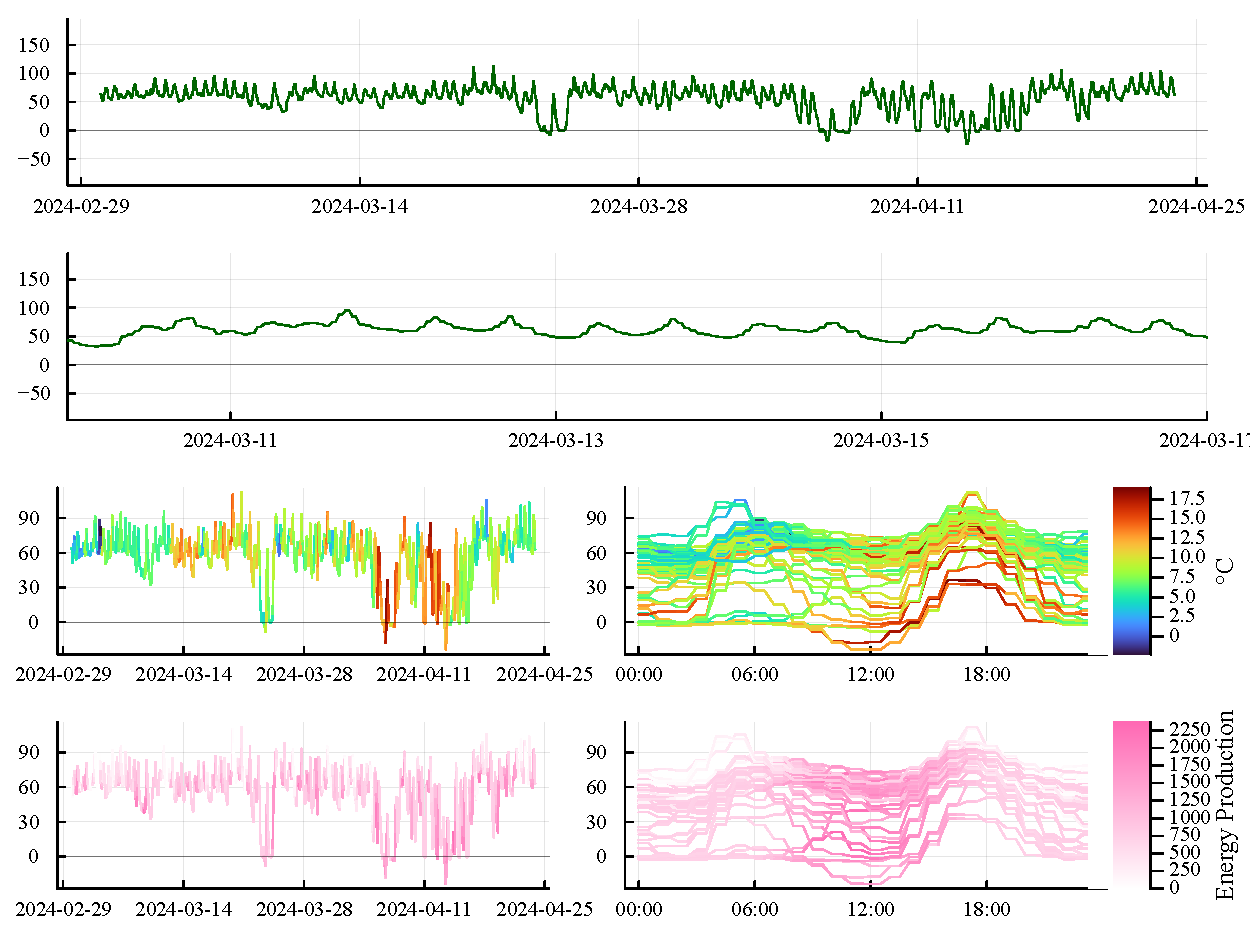
\includegraphics{EnergyProdConformalLSTM_files/mediabag/EnergyProdConformalLSTM_files/figure-pdf/monthly-dap-energy-price-plots-output-1.pdf}

}

\caption{\label{fig-monthly-dap-energy-price-plots}Day Ahead Prices.
Top: complete time history. Middle: one-week history. Bottom Left: price
history vs.~temperature (top) and total energy production (bottom).
Bottom right: daily seasonality of price vs.~temperature (top) and total
energy production (bottom).}

\end{figure}%

We see different characteristics with the SSP plots in
Fig.~\ref{fig-monthly-ssp-energy-price-plots} as the signal is hardly
distinguishable from a random walk. The domain of the SSP is The SSP is
a different story as the time series is twice that of the DAP and it
traverses from low values to high values in cycles that are not obvious.
The only seasonality observed is that around 18:00, the SSP typically
constricts to a range between about 25 and 100. The curves themselves
look like spaghetti which further indicates that the change in SSP is
practically random. As mentioned above, if the SSP became predictable,
the market would eliminate the arbitrage opportunity.

\begin{figure}

\centering{

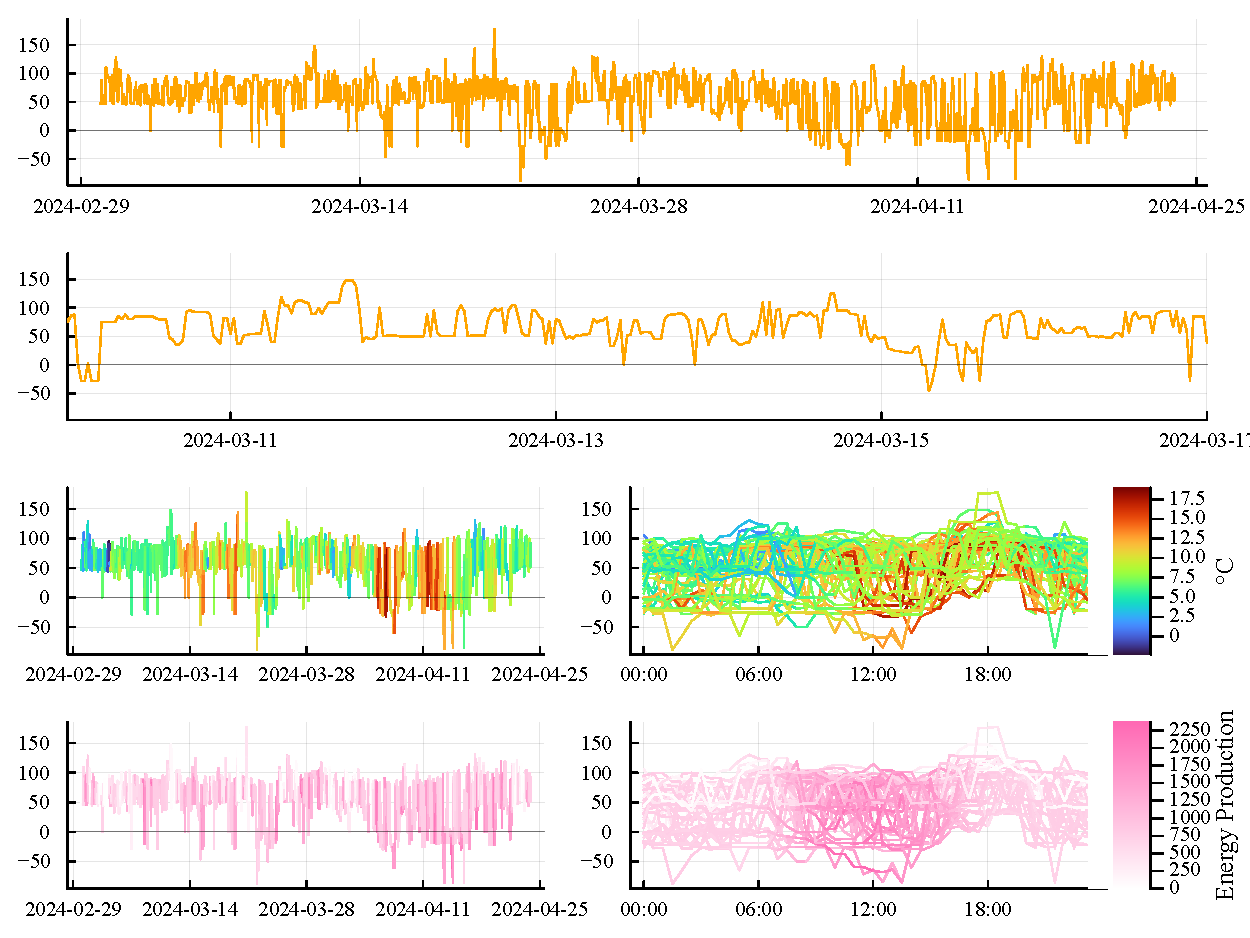
\includegraphics{EnergyProdConformalLSTM_files/mediabag/EnergyProdConformalLSTM_files/figure-pdf/monthly-ssp-energy-price-plots-output-1.pdf}

}

\caption{\label{fig-monthly-ssp-energy-price-plots}Single Settlement
Prices. Top: complete time history. Middle: one-week history. Bottom
Left: price history vs.~temperature (top) and total energy production
(bottom). Bottom right: daily seasonality of price vs.~temperature (top)
and total energy production (bottom).}

\end{figure}%

The next data visualization in Fig.~\ref{fig-violin-plots} depicts a
statistical summary of the energy production and market prices for each
day in the period as well as grouped by day of the week and hour of the
day. The violin plots indicate the density of observations near that
level for the given group. The boxplots quantify the spread by showing
the mean, quartiles, and outliers. These plots capture the trend over
the entire time and the daily seasonality better than a single time
series plot. Where before the SSP looked like a random walk, we can
observe some correlation to the DAP. Still, we note that the variance of
the SSP is much wider. The duck curve for the DAP is more pronounced and
we see there is a fairly tight first quartile, but with outliers far
beyond this range. Lastly, we note that the energy production is
somewhat random over a longer period, but fairly consistent on a daily
cycle.

\begin{figure}

\centering{

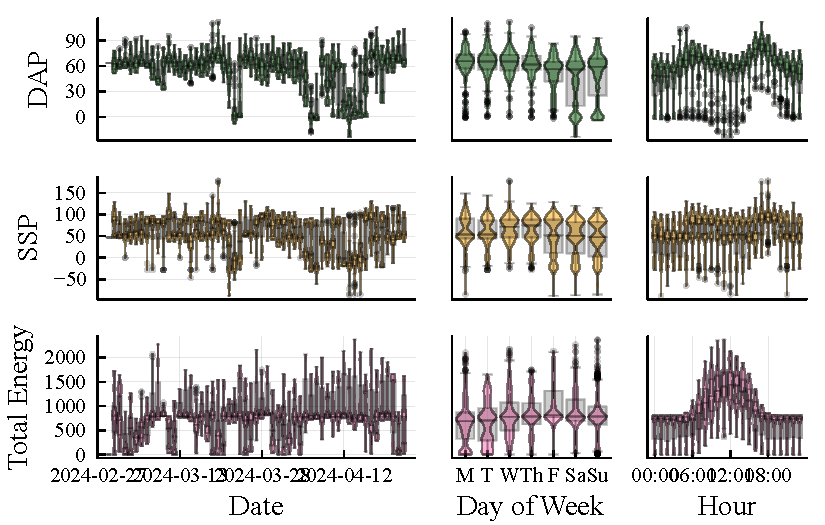
\includegraphics{EnergyProdConformalLSTM_files/mediabag/EnergyProdConformalLSTM_files/figure-pdf/violin-plots-output-1.pdf}

}

\caption{\label{fig-violin-plots}Statistical summary of the energy
production and market prices for each day in the period as well as
grouped by day of the week and hour of the day.}

\end{figure}%

The pairplot in Fig.~\ref{fig-correlation-plots} the direct correlation
or lack thereof among the key variables. Cloud cover is not a strong
indicator for two reasons. First, it would have the strongest impact on
the system during the daytime only. Second, it is an asymmetric feature
skewed towards very cloudy. Windspeed is a strong predictor of total
energy as expected and there is a negative trend between total energy
production and market prices. This indicates that our system is not an
outlier from others in this grid as all correlations are as expected.

\begin{figure}

\centering{

\includegraphics{EnergyProdConformalLSTM_files/mediabag/EnergyProdConformalLSTM_files/figure-pdf/correlation-plots-output-1.pdf}

}

\caption{\label{fig-correlation-plots}Correlation PairPlot}

\end{figure}%

The group of marginal kernel density estimate (KDE) plots in
Fig.~\ref{fig-marginal-kde} offer a final visualization of the
correlation among the key features. At the top left we see a slight
positive correlation between Total Energy and Wind Speed. At the top
right, we observe that the DAP and Total Energy are perpendicular to
each other, indicating no correlation. The same observation is true for
the Total Energy and SSP in the bottom left. In the bottom right we see
two correlated regions. Most significantly, we see that the very
negative SSP prices are associated with the lowest DAP prices. Then we
see a general correlation for the main region of prices but the two
upper peaks of the SSP are independent of the DAP.

\begin{figure}

\centering{

\includegraphics{EnergyProdConformalLSTM_files/mediabag/EnergyProdConformalLSTM_files/figure-pdf/marginal-kde-output-1.pdf}

}

\caption{\label{fig-marginal-kde}Marginal KDEs. Top Left: Total Energy
vs.~Wind Speed. Top Right: Total Energy vs.~DAP. Bottom Left: Total
Energy vs.~SSP. Bottom Right: DAP vs.~SSP.}

\end{figure}%

\subsection{Data Conclusions}\label{data-conclusions}

The analysis of the time series and correlations among the data support
our hypothesis that there are predictable dynamics at play which would
allow for accurate predictions. However, the dynamics are not
straightforward and highly nonlinear. We consider this system to be an
ideal one to model with a neural network as it can approximate any
function. While we lose explainability and we are only left with a point
forecast, we can use the methods mentioned at the outset to use the
predictions in probabilistic trading strategies. The next section will
detail the LSTM model we used to make these predictions.

\section{Long Short-Term Memory
Model}\label{long-short-term-memory-model}

We implemented an LSTM recurrent neural network (RNN) multi-target
regressor to predict the solar, wind, total energy, DAP, and SSP for the
next time step. We selected an LSTM over a generic RNN or Gated
Recurrent Unit (GRU) because LSTMs solve the so-called vanishing
gradient problem associated with generic RNN but still exhibit longer
``memory'' of past events compared to GRUs. The complex dynamics among
the features can be approximated by the dense output layer. Outputting
all targets at once is computationally efficient and provides the model
with additional information when updating the parameters. The
seasonality of the solar production and DAP were provided directly a
sinusoidal waves with periods of 24 hours and 12 hours, respectively.
All inputs and outputs were normalized so that the different scales of
the multi-target regression targets would not affect the model's
learning.

\subsection{Training}\label{training}

We used Julia's deep learning library, Flux
\citeproc{ref-Flux.jl-2018}{{[}6{]}}, to build and train the LSTM. The
workflow is as follows:

\begin{enumerate}
\def\labelenumi{\arabic{enumi}.}
\tightlist
\item
  Define the loss function. We used mean squared error as we wanted to
  penalize outliers.
\item
  Build the LSTM. Our LSTM consists of two LSTM layers followed by a
  dense output layer with a sigmoid activation. The input size, twelve,
  is the length of the weather and energy columns plus two for the
  seasonality components. The output length, five, is the length of the
  energy columns. The hidden dimension size is eight. This results in a
  model with 1,293 trainable parameters.
\item
  Set up the optimizer. We used the Adam optimizer with a learning rate
  of 1e-4.
\item
  Train the model on the training data. A special note for training
  LSTMs is that it can be important to reset the LSTM and then call it
  on the first batch of data before training it on the subsequent
  batches. This primes the LSTM's hidden state so that gradients are
  based on the recent data and not some arbitrary state. We trained the
  model for 128 epochs on 45\% of the available data with batch sizes of
  32.
\end{enumerate}

\subsection{Performance}\label{performance}

We simulated the trading environment by making predictions up to 48
hours out from a given time. For instance, we would run the model on
data up to 8:00 AM on Monday, the time at which we must submit bids for
the period of 8:30 AM Tuesday to 8:00 AM Wednesday. Beginning at 8:30 AM
on Monday, the model pulls ``forecasted'' weather data and its own
latest predictions to predict the next outputs. This continues until the
prediction period is complete. We observe the performance on the testing
data below.

Qualitatively, we observe the LSTM predictions in
Fig.~\ref{fig-predictions} are sensible and follow the general
characteristics of the target variables. The predicted values are
plotted in color over the actual values in grey. The solar and wind
predictions capture the general moving average but are not as accurate
individually as the total energy predictions. The DAP prediction also
generally captures the trend and seasonality of the actual values. The
SSP predictions are, as expected, less precise than the other
predictions. It is unable to capture the random fluctuations in the
values but it stays in the general range of the actual values.

\begin{figure}

\centering{

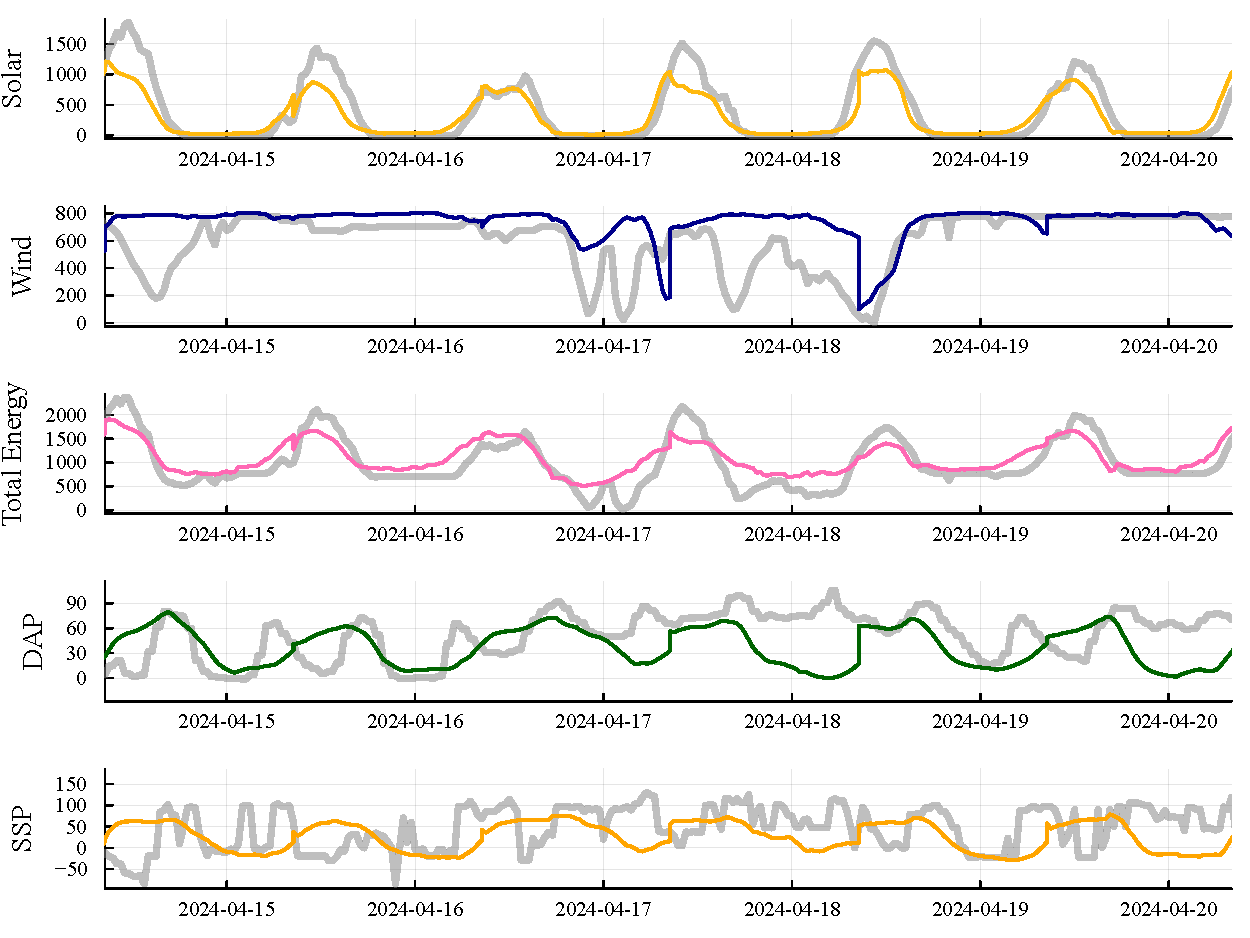
\includegraphics{EnergyProdConformalLSTM_files/mediabag/EnergyProdConformalLSTM_files/figure-pdf/plot-predictions-output-1.pdf}

}

\caption{\label{fig-predictions}Test Data Predictions}

\end{figure}%

We check the Mean Absolute and Root Mean Squared Error for all three
testing sets to ensure the model is not overfitting. The results are
shown in Table~\ref{tbl-MAE-error} and Table~\ref{tbl-RMSE-error}. The
error values are fairly consistent across datasets for the two error
measures indicating that we have not overfit the model. The errors are
typically worse in the test but not to the point of overfitting. More
than likely, there are some events present in the test data that are not
observed in the training data. The best way to improve this would be to
increase the history of the training data.

\begin{table}

\caption{\label{tbl-MAE-error}Mean Absolute Error}

\centering{

\phantomsection\label{test-error}
\begin{tabular}{r|cccc}
    & feature & Train & Calib & Test\\
    \hline
    & Symbol & Float64 & Float64 & Float64\\
    \hline
    1 & Solar & 148.681 & 149.791 & 210.36 \\
    2 & Wind & 181.207 & 216.488 & 193.169 \\
    3 & TotalEnergy & 294.591 & 252.243 & 318.488 \\
    4 & DAP & 17.853 & 22.0404 & 21.6718 \\
    5 & SSP & 32.5873 & 37.1497 & 41.2682 \\
\end{tabular}

}

\end{table}%

\begin{table}

\caption{\label{tbl-RMSE-error}Root Mean Square Error}

\centering{

\phantomsection\label{test-error-squared}
\begin{tabular}{r|cccc}
    & features & Train & Calib & Test\\
    \hline
    & Symbol & Float64 & Float64 & Float64\\
    \hline
    1 & Solar & 242.333 & 242.563 & 331.406 \\
    2 & Wind & 292.243 & 327.327 & 270.718 \\
    3 & TotalEnergy & 410.222 & 351.866 & 426.21 \\
    4 & DAP & 23.7798 & 28.7697 & 29.0975 \\
    5 & SSP & 41.8374 & 47.0617 & 51.722 \\
\end{tabular}

}

\end{table}%

Looking at the residual histograms in
Fig.~\ref{fig-calib-residuals-histograms}, we see they resemble Normal
distributions centered on zero. This indicates we will be able to
conformalize the model to obtain a probabilistic forecast. Solar
residuals have most values at zero because the model correctly predicts
no solar energy production at night. We get around this by using the
combined energy as we don't explicitly have to know the solar and the
wind energy production.

\begin{figure}

\centering{

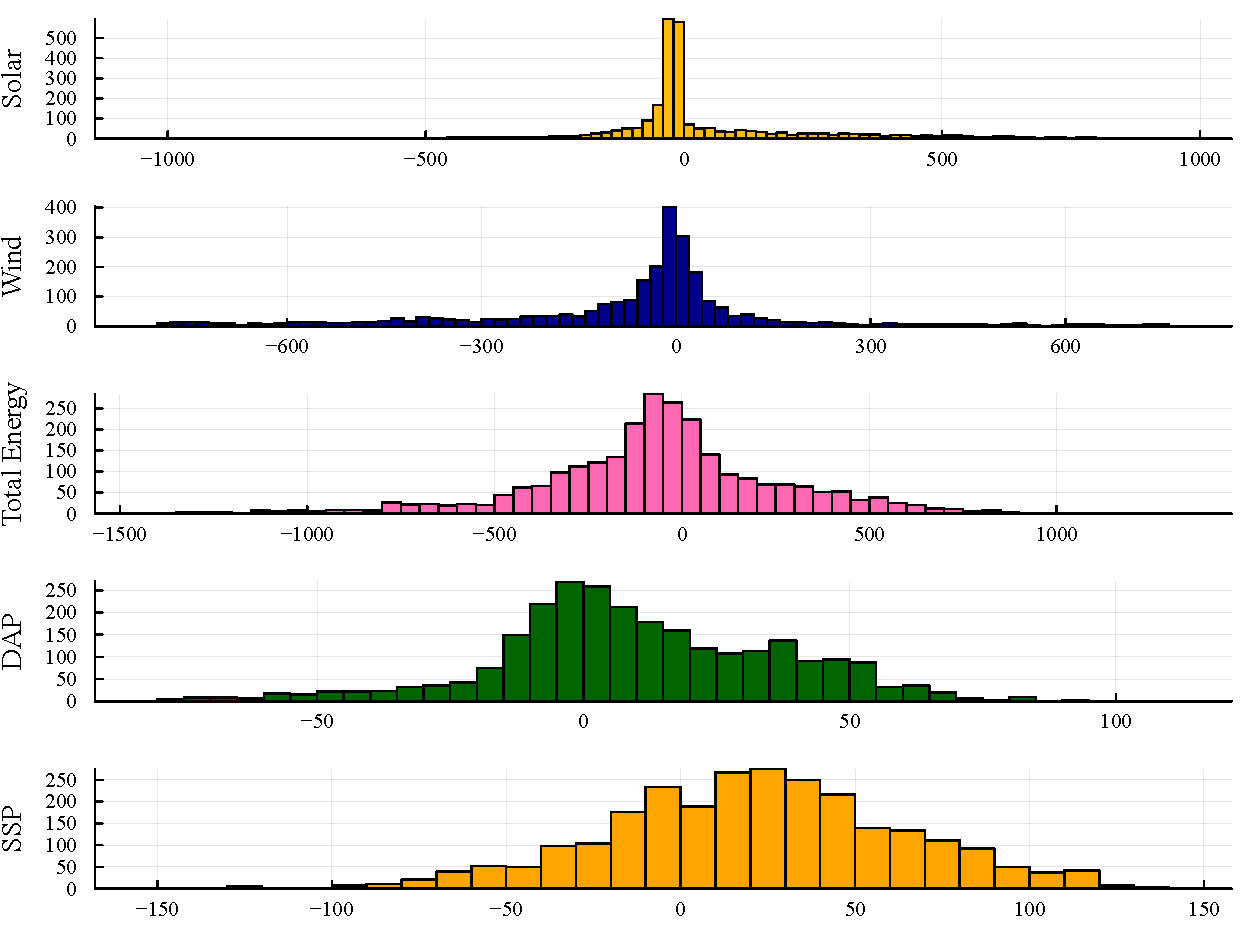
\includegraphics{EnergyProdConformalLSTM_files/mediabag/EnergyProdConformalLSTM_files/figure-pdf/plot-residuals-output-1.pdf}

}

\caption{\label{fig-calib-residuals-histograms}Calibration Data
Residuals}

\end{figure}%

\section{Conformalizing LSTM}\label{conformalizing-lstm}

We are satisfied with the performance of the LSTM, but there is an
unquantified risk in using it because it only outputs a point forecast.
Our first method to deal with this is to conformalize the model with
calibration data. This will allow us to get confidence intervals around
the prediction which can be used in many ways by the operator. This is a
powerful and simple method to extend the utility of a model like the
LSTM.

\subsection{Implementation}\label{implementation}

The process is essentially accomplished in two steps. First,
non-conformity scores are calculated for each prediction in the
calibration data. Second, a desired quantile is retrieved which
represents the probability that the true value will be within a certain
amount of non-conformity with that quantile. For our purposes,
nonconformity scores are just the mean error and they are indexed by
time.

\subsection{Performance}\label{performance-1}

The heatmaps in Fig.~\ref{fig-nonconformity-heatmaps} show the
non-conformity of the Total Energy, DAP, and SSP show the results. The
x-axis is the time of day, and the y-axis is the probability of the true
value being within the non-conformity score indicated by the color bar.
Blue values are desirable as they indicate a low non-conformity score
while red indicates a high non-conformity score. For instance, at 3:00
AM, the Total Energy score was low with a value of around 200 with
probability 1. So we can be very confident the true value will be within
200 MWh of the prediction. Conversely, the DAP at 7:00 AM has a
relatively high non-conformity score that dips down below the 0.5
quantile. This means that we cannot even be sure that true DAP will be
within 40 GBP/MWh with better than 50\% probability.

\begin{figure}

\centering{

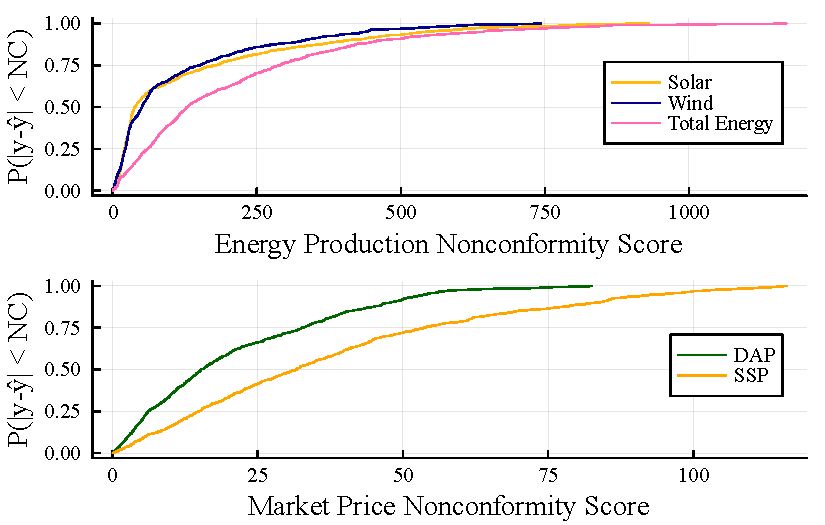
\includegraphics{EnergyProdConformalLSTM_files/mediabag/EnergyProdConformalLSTM_files/figure-pdf/plot-nonconformity-output-1.pdf}

}

\caption{\label{fig-nonconformity-heatmaps}Nonconformity Scores
Probabilities}

\end{figure}%

\section{Market Trading}\label{market-trading}

The predictions of the energy production and market prices are used to
inform the bidding for the following day using different strategies for
comparison. The operator cannot store energy or commit to negative
energy production. The strategies explored are:

\begin{enumerate}
\def\labelenumi{\arabic{enumi}.}
\tightlist
\item
  Commit the Point Forecast
\item
  Commit the Point Forecast - a 10\% confidence interval obtained from
  Conformal Prediction
\item
  Conditional Value at Risk
\end{enumerate}

These strategies are compared to a benchmark of the revenue generated
from perfectly predicting and committing the total energy produced. We
consider this to be the most reasonable benchmark as anything better
amounts to timing the SSP market. Revenue is calculated for this
competition according to this formula(\ref{eq-revenue}) which
approximates the impact of the difference between the energy prediction
and actual production on the settlement price.

\begin{equation}\phantomsection\label{eq-revenue}{
Revenue = Trade*DAP + \Delta_E (SSP - 0.07 \Delta_E)
}\end{equation} \[
\Delta_E = Actual - Trade
\] The difference between actual and traded energy is penalized by the
SSP and its square multiplied by \(0.07\). This is the piece that
penalizes for both over and underproduction when SSP is positive which
is the norm. While there are times when SSP is negative, they tend to be
at times of overproduction so there is not a realistic way to exploit an
arbitrage scenario by over-promising and under-delivering during such
periods.

\subsection{Revenue from Point
Prediction}\label{revenue-from-point-prediction}

The predicted total energy is used as the traded amount in the day ahead
market. Revenue is calculated as shown above using the actual total
energy and the actual market prices. This does not consider the
forecasts for the market prices and is the most straightforward to
implement. Since there is no quantification of risk, there is no
indication of the expected value of this energy commitment or possible
undesirable outcomes.

\subsection{Revenue from Conformal
Prediction}\label{revenue-from-conformal-prediction}

We concluded that as a general rule, it is possible to reduce risk by
under-committing energy rather than over-committing in the day-ahead
market. The revenue formula penalizes failing to meet the commitment
more. It is a delicate balance and we found that reducing the point
prediction by the non-conformity score at the 10\% quantile can have a
favorable impact on the revenue. This approach could be justified by a
game-theory approach which would consider playing the game indefinitely.
Currently, this value is arbitrary without a strong justification but is
included as an example of how the conformal prediction can and cannot be
used.

\subsection{Revenue from Conditional Value at
Risk}\label{revenue-from-conditional-value-at-risk}

\subsubsection{Overview}\label{overview}

Stochastic optimization of the trade decisions using Conditional Value
at Risk allows us to consider aspects that the point prediction and CP
method cannot. Specifically, the trade decision can be optimized
directly for revenue outcomes while considering uncertainties. This also
requires the uncertainties of the market prices to be treated as well.
This additional context results in a defensible strategy that can
optimize an operator's trading strategy within a specified risk
tolerance.

For this strategy, we assume we are risk averse and our goal is to
maximize the expected value of some lower quartile of possible outcomes.
In this study, we opted for 33\% to indicate that more likely than not,
in the worst 33\% of cases, we will have a certain amount of revenue.
This is a more sophisticated method than the previous two and is a more
realistic representation of the trading environment. Future work could
include a specific risk profile that would specify that, for example,
the probability of losing X in any one time period or day must be less
than Y\% or the probability of ever falling below a certain threshold
must be less than Z\%.

\subsubsection{Implementation}\label{implementation-1}

We implemented CVaR by sampling residuals from the calibration data and
adding them to the point forecast. At each prediction step we did the
following:

\begin{enumerate}
\def\labelenumi{\arabic{enumi}.}
\tightlist
\item
  Sample 250 residuals from the calibration data. These are indexed by
  time which captures two key elements simultaneously. First, is that
  the model may just be more accurate for a given feature at some time.
  This could be based on weather patterns, demand, or any number of
  factors. Secondly, it captures that at the 9:00 AM prediction, we are
  only 49 steps into the future while at the 7:30 AM prediction, we are
  at 97 steps. We know that error accumulates over time so this is an
  important factor to consider.
\item
  Add the residuals to the point forecast to get 250 scenarios of the
  total energy, DAP, and SSP.
\item
  Evaluate the revenue gained for each scenario at all available trade
  amounts. The true energy production is taken as the point forecast
  plus the scenario energy production residual.
\item
  At each available trade amount, calculate the mean of the lower 33\%
  of the revenues in the scenarios. This is the CVaR.
\item
  Find the trade amount with the maximum CVaR.
\end{enumerate}

The results of this process are depicted in Fig.~\ref{fig-cvar-plot}.
The multi-colored curves represent different scenarios evaluated for
each available trade amount. The color represents how far off the
predicted energy production was from the actual energy production. The
solid black curve is the mean, or expected value of trading that amount
of energy for those scenarios. The dashed black curve is the CVaR. For
this optimization problem with a single decision variable, how much to
trade, we can graphically see the maximum is at about 700 MWh. So the
decision is made to trade that amount and the actual revenue is shown as
the green diamond. Also plotted are the ``+'' showing the revenue from a
perfect prediction and commitment of the energy production and the ``o''
showing the point prediction and associated revenue. The fact that the
CVaR revenue is higher than the CVaR curve shows that the actual revenue
cannot be known, and that CVaR curve is just the expected value of that
quantile. In this case, the maximal CVaR happens to be close to the
maximal mean, but it is not always the case. Typically, we would see the
CVaR peak at a point off of the peak of the mean curve. The goal is to
maximize the expectation of the worst outcomes, but this comes at the
cost of not maximizing the outcome. If one had infinite funds and could
assume infinite risk, the optimal strategy would be to maximize the
expected value. In the real world, we prefer to limit our risk exposure.
Lastly, we note that CVaR performs better than the point forecast. With
CVaR we have accounted for our uncertainty about the energy production
and market prices while the point forecast is only considering
production and no uncertainty. This highlights the importance of
considering the uncertainty in the predictions and trading.

\begin{figure}

\centering{

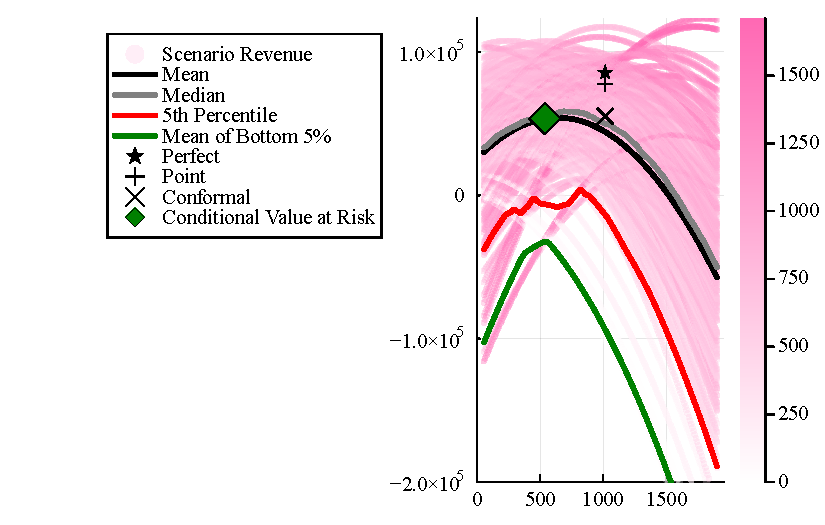
\includegraphics{EnergyProdConformalLSTM_files/mediabag/EnergyProdConformalLSTM_files/figure-pdf/cvar-plot-example-output-1.pdf}

}

\caption{\label{fig-cvar-plot}Conditional Value at Risk Example
(2024-04-14 22:30)}

\end{figure}%

\subsection{Performance}\label{performance-2}

The plot of cumulative revenue over the testing period for each trading
strategy is shown in Fig.~\ref{fig-cumulative-revenue}. The perfect
forecast is a point of reference for what would be achieved if the
operator could perfectly predict the production and not trade on the
real-time market at all. As expected, this is the highest value even
though it does not consider market prices. Next, we see that CP-adjusted
commitment outperforms the other strategies. As alluded to earlier, this
may be a case of gambling and getting lucky as there is no justification
for this reduction other than that it happened to perform well.
Conversely, there may be a strong underlying reason which would explain
why this is a good strategy. Next, we see that CVaR is just behind the
CP-adjusted strategy. Lastly, the point forecast performed the worst as
it suffered the biggest loss in the first week and never fully recovered
to the level of the other two strategies.

\begin{figure}

\centering{

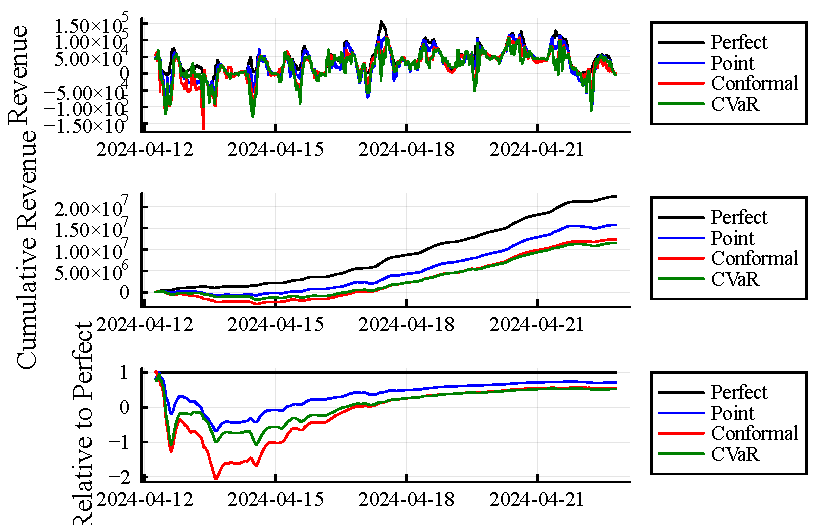
\includegraphics{EnergyProdConformalLSTM_files/mediabag/EnergyProdConformalLSTM_files/figure-pdf/revenue-plots-output-1.pdf}

}

\caption{\label{fig-cumulative-revenue}Test Data Cumulative Revenues}

\end{figure}%

\section{Conclusions}\label{conclusions}

The revenue from all three strategies built from the LSTM are on the
same order of magnitude and off by a factor of two from the perfect
energy production revenue. This indicates that our model and strategies
are promising in their ability to capture the highly nonlinear and
complex dynamics of the system, time dependency, and uncertainties. It
also indicates there is room for improvement. We have identified the
areas below as good places to start for future work:

\begin{enumerate}
\def\labelenumi{\arabic{enumi}.}
\tightlist
\item
  Incorporate more data. We have purposely used a small subset of the
  available data sources, features, and history to build and test this
  model as a simplistic starting point and proof of concept.
  Specifically, demand forecasts and weather from more nearby locations
  would be useful.
\item
  Feed longer sub-sequences to the LSTM. Currently, the LSTM is updating
  its state only on the last step and then predicting the next step. It
  would be better to provide a lookback window of at least 24 hours so
  the seasonality would be learned implicitly rather than provided
  explicitly.
\item
  Predict optimal (or near-optimal) trade amounts directly. Once
  forecasts have been created for the features, train a model that takes
  those probabilistic forecasts to predict the optimal trade amount.
  This may offer a more direct path to maximizing revenue, although it
  would not be explainable as CVaR or other strategies are.
\item
  Test the CVaR on different risk profiles.
\end{enumerate}

The problems addressed in this study are practical, real-world decisions
that renewable energy production operators must answer every day. This
report shows how advanced technologies and methodologies that rely on
probabilistic approaches are within reach and can be used to limit risk
for these operators. In the long run, reducing this risk will make
investment in renewable energy more palatable and bring more systems
online which will be a net benefit for the environment and the economy.

\phantomsection\label{refs}
\begin{CSLReferences}{0}{0}
\bibitem[\citeproctext]{ref-ieeehybridcomp}
\CSLLeftMargin{{[}1{]} }%
\CSLRightInline{{``Hybrid energy forecasting and trading competition.''}
IEEE DataPort {[}Online{]}. Available:
\url{https://ieee-dataport.org/competitions/hybrid-energy-forecasting-and-trading-competition}}

\bibitem[\citeproctext]{ref-DBLP:journalsux2fcorrux2fabs-2107-07511}
\CSLLeftMargin{{[}2{]} }%
\CSLRightInline{A. N. Angelopoulos and S. Bates, {``A gentle
introduction to conformal prediction and distribution-free uncertainty
quantification,''} \emph{CoRR}, vol. abs/2107.07511, 2021 {[}Online{]}.
Available: \url{https://arxiv.org/abs/2107.07511}}

\bibitem[\citeproctext]{ref-Xu2020-ib}
\CSLLeftMargin{{[}3{]} }%
\CSLRightInline{W. Xu, P. Zhang, and D. Wen, {``Decision-making model of
electricity purchasing for electricity retailers based on conditional
value-atRisk in day-ahead market,''} in \emph{2020 12th {IEEE} {PES}
{Asia-Pacific} power and energy engineering conference ({APPEEC})},
2020. }

\bibitem[\citeproctext]{ref-RebaseApi}
\CSLLeftMargin{{[}4{]} }%
\CSLRightInline{{``Hybrid energy forecasting and trading competition.''}
Rebase Energy {[}Online{]}. Available:
\url{https://www.rebase.energy/challenges/heftcom2024}}

\bibitem[\citeproctext]{ref-VisualCrossing}
\CSLLeftMargin{{[}5{]} }%
\CSLRightInline{{``Weather data \& API.''} Visual Crossing {[}Online{]}.
Available: \url{https://www.visualcrossing.com/weather-api}}

\bibitem[\citeproctext]{ref-Flux.jl-2018}
\CSLLeftMargin{{[}6{]} }%
\CSLRightInline{M. Innes \emph{et al.}, {``Fashionable modelling with
flux,''} \emph{CoRR}, vol. abs/1811.01457, 2018 {[}Online{]}. Available:
\url{https://arxiv.org/abs/1811.01457}}

\end{CSLReferences}


% Can use something like this to put references on a page
% by themselves when using endfloat and the captionsoff option.
\ifCLASSOPTIONcaptionsoff
  \newpage
\fi

% trigger a \newpage just before the given reference
% number - used to balance the columns on the last page
% adjust value as needed - may need to be readjusted if
% the document is modified later
%\IEEEtriggeratref{8}
% The "triggered" command can be changed if desired:
%\IEEEtriggercmd{\enlargethispage{-5in}}

% Uncomment when use biblatex with style=ieee
%\renewcommand{\bibfont}{\footnotesize} % for IEEE bibfont size

\pagebreak[3]
% that's all folks
\end{document}

